\documentclass[12pt]{article}
\usepackage[english]{babel}
\usepackage{float}
\usepackage[margin=1in]{geometry}
\usepackage{graphicx}
%\usepackage[toc,page]{appendix}
\graphicspath{ {./img/} }
\newcommand{\rpm}{\raisebox{.2ex}{$\scriptstyle\pm$}} 
\usepackage{listings}
\usepackage{xcolor}
\usepackage{indentfirst}
\usepackage{caption}
\usepackage[final]{pdfpages}


\begin{document}

\title{Joe Phaneuf \\ Computer Vision 16-720 Spring 2018 Homework 3 \\ Mar. 7, 2018 }
\date{}
\author{}
\maketitle

\newpage


%\stepcounter{section}
%%%%%%%%%%%%%%%%%%%%%%%%%%%%%%%%%%%%%%%%%%%%%%%%%%%%%%%%%%%%%%%%%%%%%%%%%%%%%%%%
%%%%%%%%%%%%%%%%%%%%%%%%%%%%%%%%%%%%%%%%%%%%%%%%%%%%%%%%%%%%%%%%%%%%%%%%%%%%%%%%
\section{Q1}
\subsection{Q1.1}
In training deep networks, a ReLU activation can be chosen over a sigmoid as it is easily differentiable, and does not suffer slow training due to saturation.

\subsection{Q1.2}
Consider a one layer network with weights $W^{1}$ , bias $b^{1}$ , input $X$ and activation function $g$. The output of this network is 
$$
out^{1} = g( W^{1} X + b^{1} )
$$
if g is a linear operator function, then there will be some modified weights and biases such that
$$
out^{1} = \hat{W}^{1} X + \hat{b}^{1}
$$

For a subsequent layer, the pre-activation is
$$
W^{2} ( \hat{W}^{1} X + \hat{b}^{1} ) + b^{2}
$$
Which, due to the properties of matrix multiplication, can be reduced to some modified weights and biases
$$
\hat { W^{2} } X + \hat { b} ^{2}
$$

$\hat { W^{2} }$ and $\hat { b} ^{2}$ are of the same dimension as $W^{1}$ and $b^{1}$, meaning no additional discriminatory information can be encapsulated by the second layer. 

A non-linear activation function makes it impossible to combine weights as demonstrated above, meaning each additional layer does add to the discriminatory power of the network.

\section{Q2}
\subsection{Q2.1.1}
Weight initialization is an important factor for training neural networks. Naively initializing weights to zero results in zero valued gradients, which prevents weight updates. Initializing with all equal weights also reduces the same gradients for each weight, so training does not function properly. 

\subsection{Q2.1.3}
I chose to initialize weights from a uniform distribution ranging from -0.1 to 0.1. This was mostly from research and some experimention. Weights that are too large can create issues by way of massive gradients, weights that are too small can take a long time to train due to very small gradients.


\subsection{Q2.4.1}
Stochastic gradient descent is more robust to non-convex error manifolds , but may take longer to reach minima. Batch gradient descent will typically converge faster given error manifolds that are reasonably convex , but can be more expensive in terms of required RAM.

\section{Q3}
\subsection{Q3.1.1}
Figure \ref{fig:accloss} shows the training and validation accuracy and loss while training on the nmist26 dataset.
\begin{figure}[H]
\centering
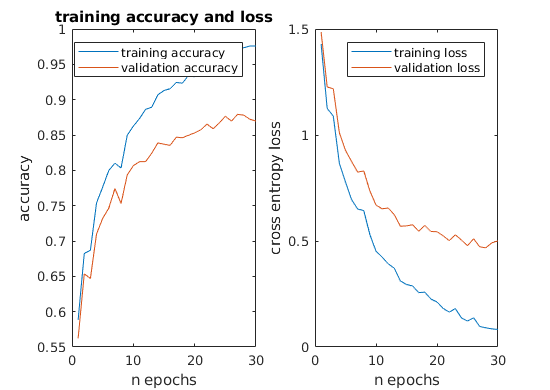
\includegraphics[page=1,width=0.4\textwidth]{q311}
\caption{Training and validation accuracy and loss} 
\label{fig:accloss}
\end{figure}   

\subsection{Q3.1.2}
Figure \ref{fig:accloss} above shows accuracy and loss for a learning rate of 0.01.  Figure \ref{fig:accloss001} shows accuracy and loss for a learning rate of 0.001.
The higher learning rate of 0.01 performed better over 30 epochs, reaching a validation accuracy of 87 percent. versus the lower learning rate which achieved a validation accuracy of 73 percent. It is interesting to note that the accuracy and loss at the higher rate appear noisier. I suspect that too high of a learning rate could become problematic because of that.
\begin{figure}[H]
\centering
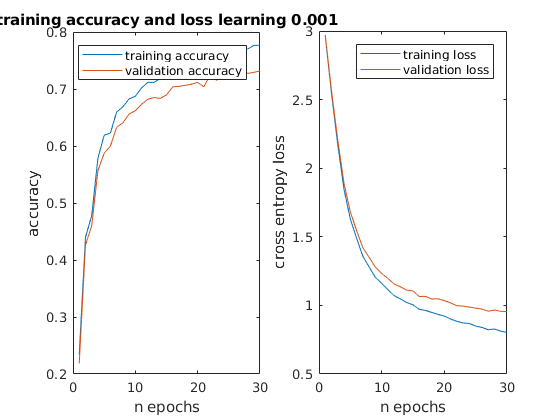
\includegraphics[page=1,width=0.4\textwidth]{q312}
\caption{Training and validation accuracy and loss} 
\label{fig:accloss001}
\end{figure}   

\subsection{Q3.1.3}
As reported in section Q3.1.1 , this neural network provided the best valiation accuracy over 30 epochs using a learning rate of 0.01. Applying this network to the nist26 test data set resulted in 88.5 percent accuracy and a average cross entropy loss of 0.5. Figure \ref{fig:weightviz} shows an image montage of weights in the first layer of this network. The first layer has 400 sets of 1024 length weight vectors.

Figure \ref{fig:initweightviz} shows the same montage with the weights initialized prior to training. The weights were initialized from a uniform distribution, and image appears to be white noise, which makes sense.

The learned weights clearly pick up on features that correspond to features of the training data set.
\begin{figure}[H]
\centering
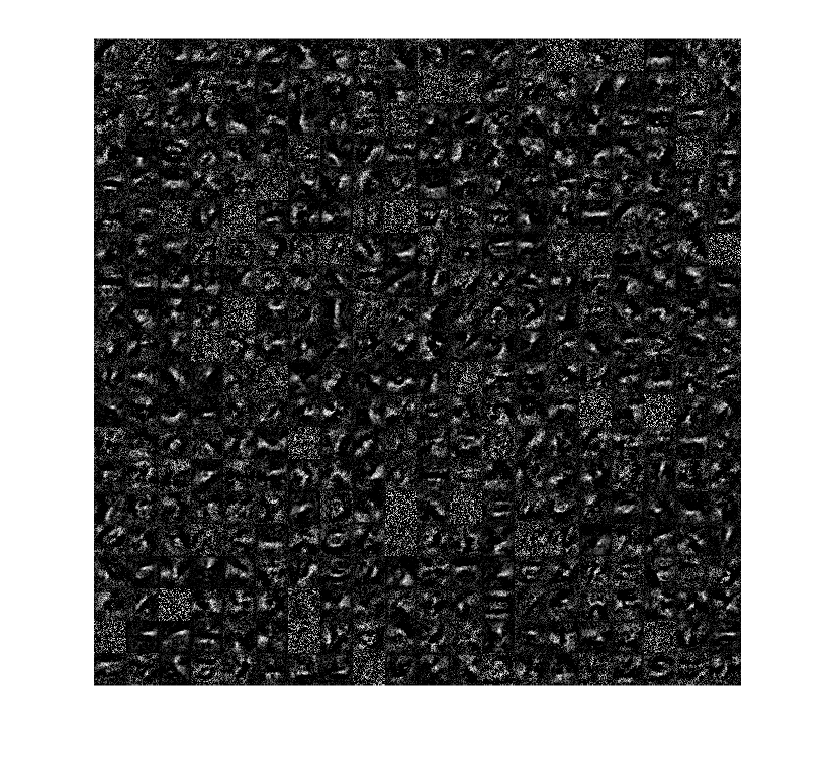
\includegraphics[page=1,width=0.4\textwidth]{weight_montage}
\caption{Visual montage of first layer weights after training} 
\label{fig:weightviz}
\end{figure}   

\begin{figure}[H]
\centering
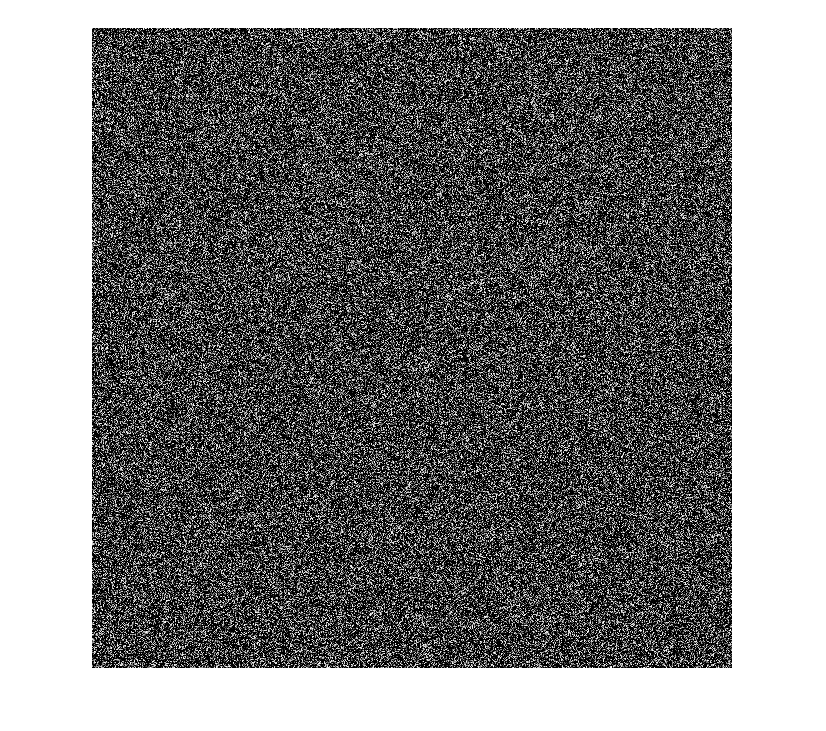
\includegraphics[page=1,width=0.4\textwidth]{init_weight_montage}
\caption{Visual montage of initial first layer weights } 
\label{fig:initweightviz}
\end{figure}   

\subsection{Q3.1.4}
Figure \ref{fig:initweightviz} shows a graphical confusion matrix for the nist26 test data. Correct predictions are shown in blue, incorrect predictions are shown in red. Each point is plotted with a low alpha, so darker points show higher frequency of occurence. This indicates that the most problematic classifications were predicting I for a true label of Z , and predicting an O for a true label of D. Honestly, I have trouble with that myself, so I can't be mad at my neural net on this one.

\begin{figure}[H]
\centering
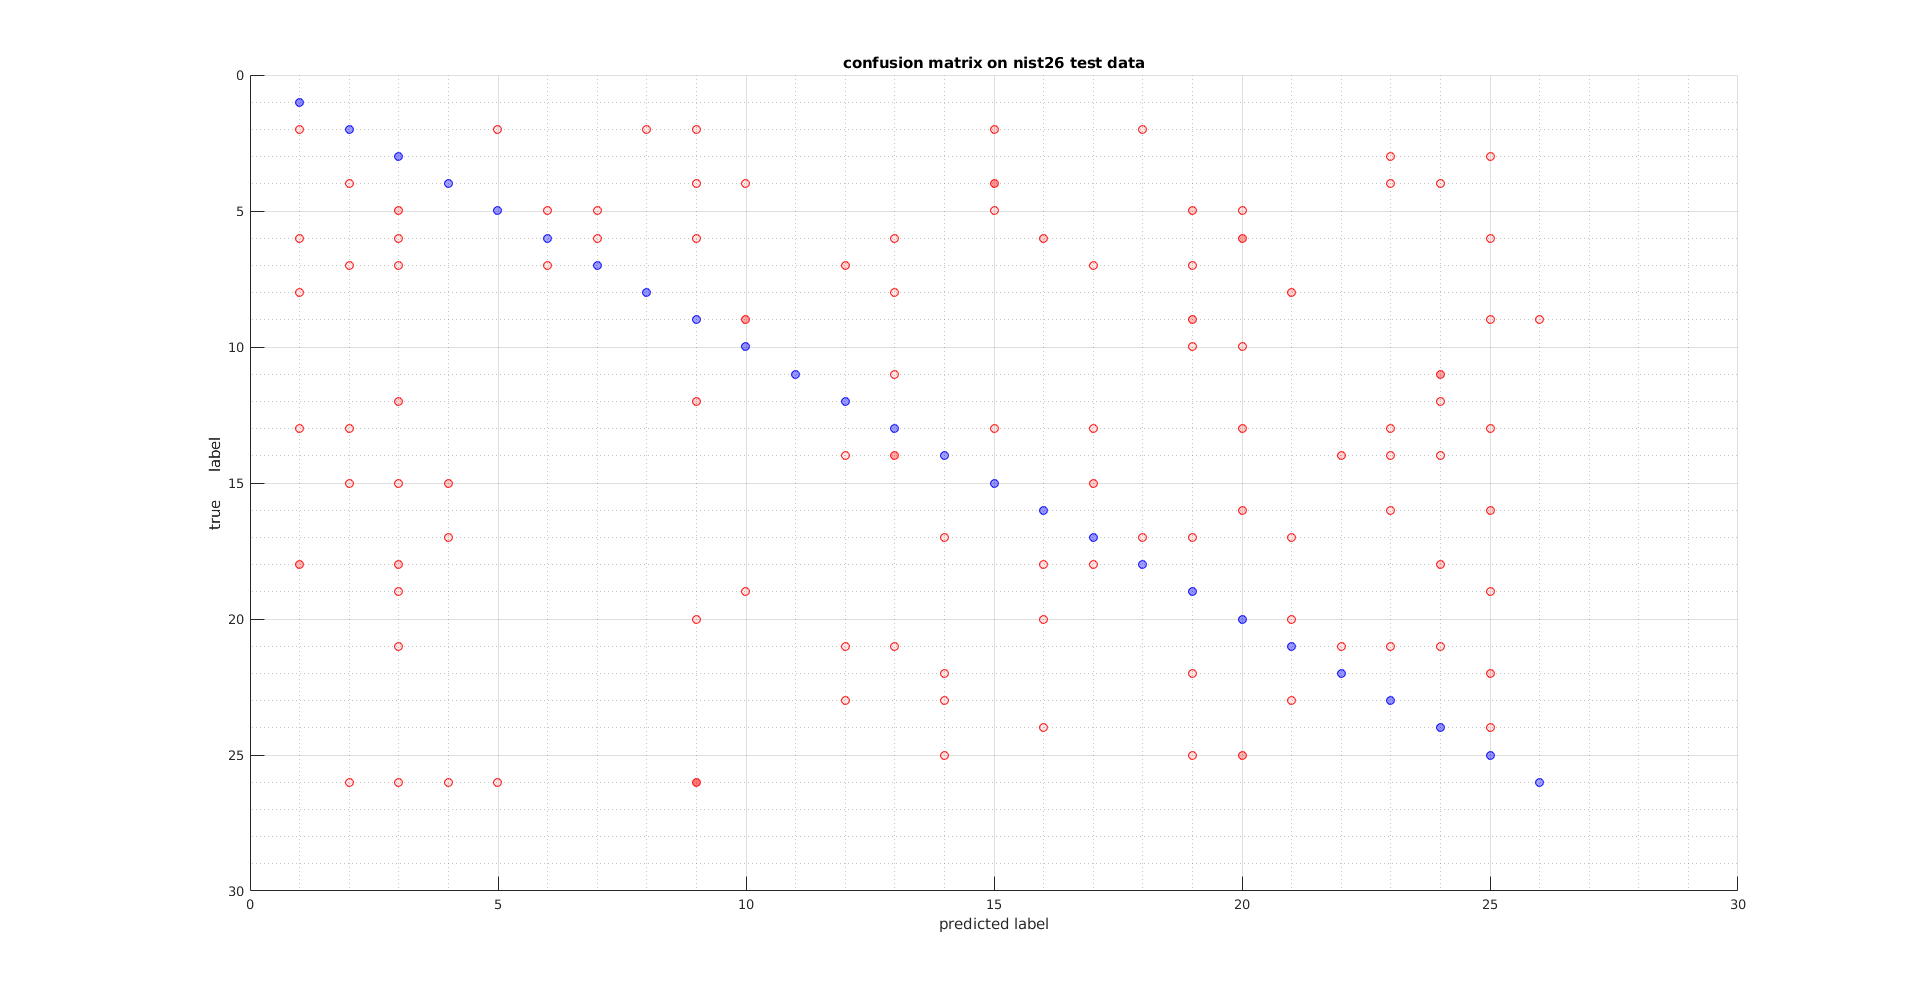
\includegraphics[page=1,width=0.75\textwidth]{q314confusion}
\caption{ Confusion matrix for test data } 
\label{fig:initweightviz}
\end{figure}   

\subsection{Q3.2.1}
\subsection{Q3.2.2}
Figure \ref{fig:nist36preweights} shows the nist36 net's first layer weights after being initialized from nist26model60iters. Figure \ref{fig:nist36retrainweights} shows the net's first layer weights after retraining with hand drawn numbers in addition to letters.
Each weight image is different, in some cases only slightly different. This is, however, difficult to parse with a feeble human brain. I was unable to pick out distinct features that are clearly associated with numbers.
Applying the retrained net to the nist36 test data resulted in an accuracy of 78 percent and a loss of 0.71
\begin{figure}[H]
\centering
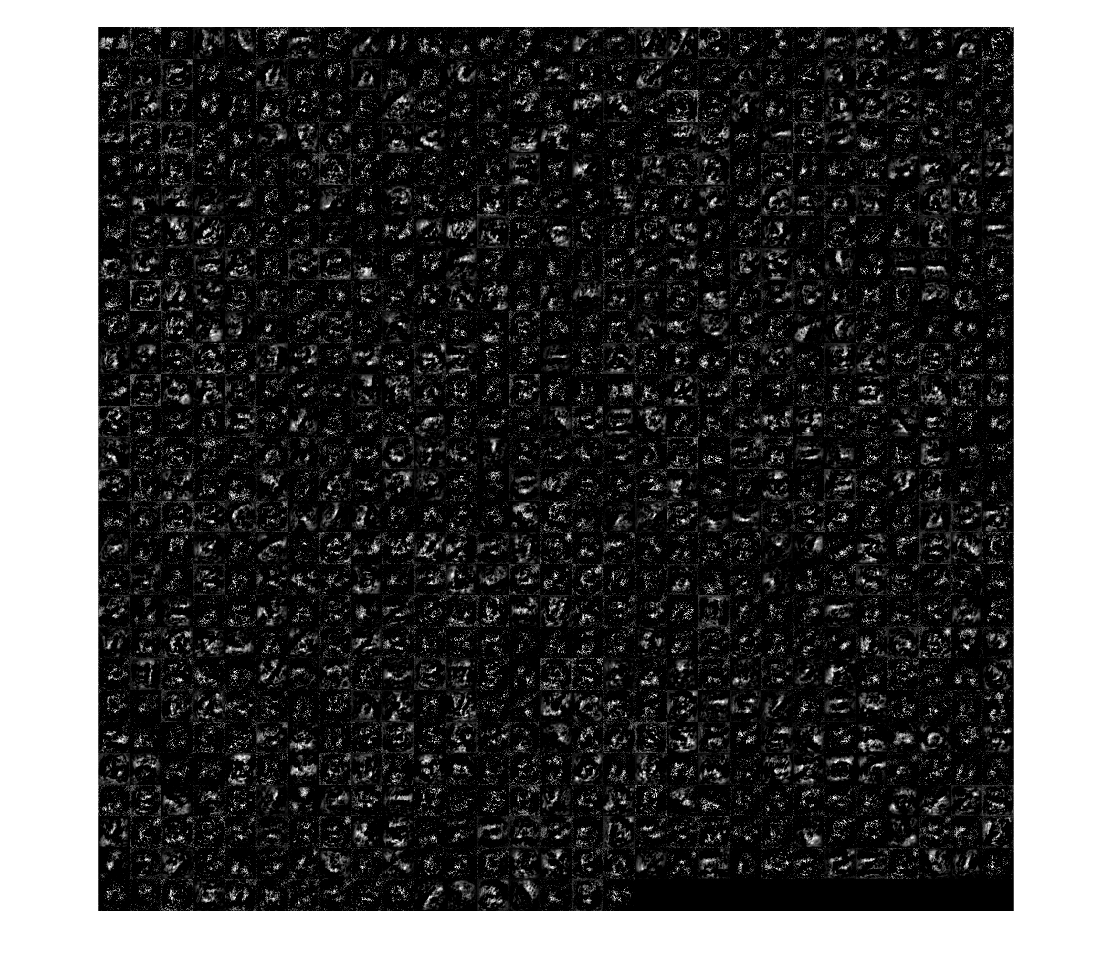
\includegraphics[page=1,width=0.75\textwidth]{q322_pre}
\caption{ Visual montage of nist26 pre-trained weights } 
\label{fig:nist36preweights}
\end{figure}   

\begin{figure}[H]
\centering
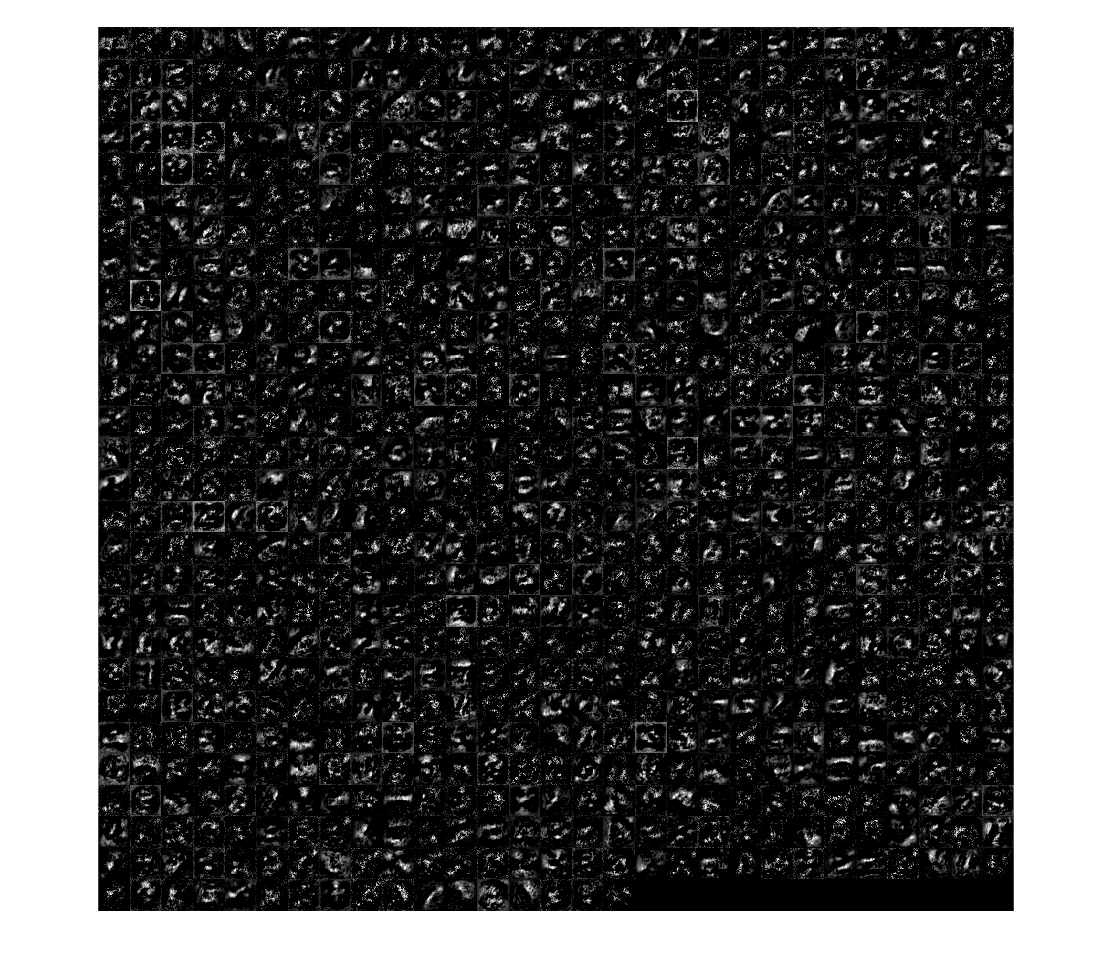
\includegraphics[page=1,width=0.75\textwidth]{q322_retrain}
\caption{ Visual montage of nist26 weights after retraining } 
\label{fig:nist36retrainweights}
\end{figure}   

\subsection{Q3.2.3}
Adding more classes to the neural net made classification more difficult and resulted in a decrease in test accuracy as compared to the nist26 data set performance. A confusion matrix for the nist36 performance is shown in Figure \ref{fig:nist36confusion}. The confusion matrix shows that this net often predicts an S for a true label of 5 , and also frequently predicts a 0 for a true lable of O. The latter is confusing for humans, and is really humanity's fault for picking symbols that look alike.
\begin{figure}[H]
\centering
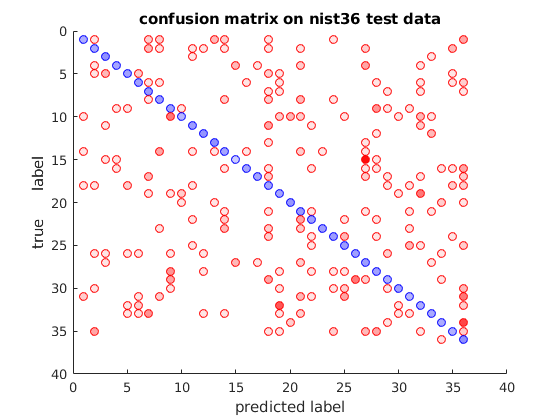
\includegraphics[page=1,width=0.75\textwidth]{q323confusion}
\caption{ Confusion matrix for nist36 test data } 
\label{fig:nist36confusion}
\end{figure}   

\section{Q4}
\subsection{Q4.1}
The character extraction technique we will employ has a makes some assumptions for the sake of simplicity, but these assumptions will result in occasional errors. This method makes an assumption that the text will be dark and background light, which may not be the case. This method also assumes that characters will be laid out left to right on horizontal lines, which will not always be the case. Another critical assumption is that only valid characters are present, so punctation or other non-character markings may cause errors.
https://stackoverflow.com/questions/43888023/how-to-extract-text-from-image-in-java
https://www.welovesolo.com/sport-elements-text-mix-vector/

\section{Q5}
\subsection{Q5.1}
Using the default settings, I noticed that the autoencoder was unable to converge. With a tweak to the learning rate, the loss and RMSE decreased for 3 epochs, but not close enough to desired RMSE. 

\subsection{Q5.2}
To drive the error lower, I adjusted the weights in the conv2D weight initialization to a standard deviation of 0.5, adjusted the learning rate to 5e-4 , applied L2 regularization with value 1e-2, and dropped the mini batch size to 5. Figure \ref{fig:nist36confusion} shows the loss and RMS error over 3 epochs of training.

\begin{figure}[H]
\centering
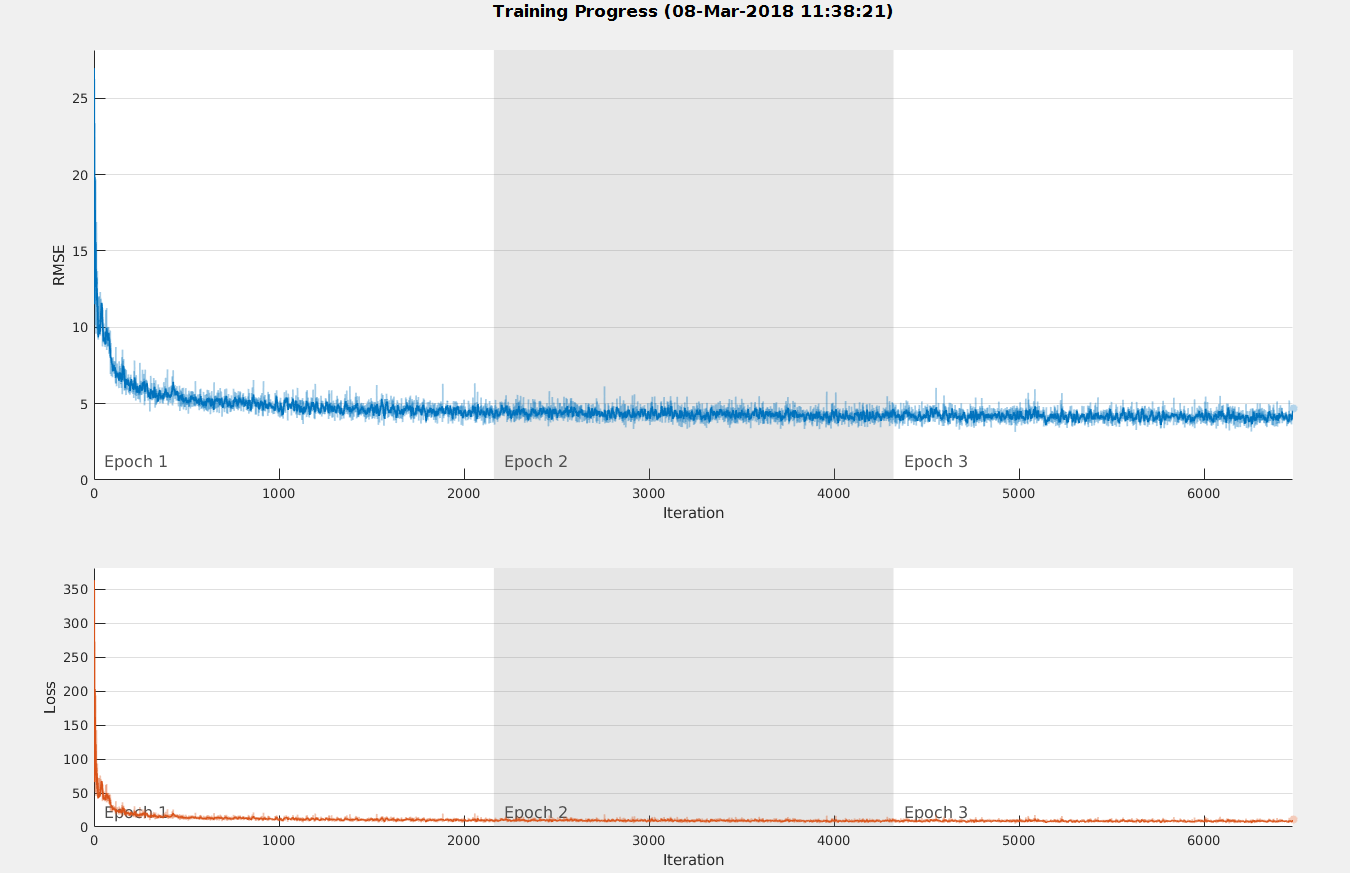
\includegraphics[page=1,width=0.75\textwidth]{q522_mrse4}
\caption{ Loss and RMSE for autoencoder training } 
\label{fig:nist36confusion}
\end{figure}   

\subsection{Q5.3}
The autoencoder outputs ( shown in Figure \ref{fig:autoencout} ) show noisy versions of the original input images, they are however visibly similar to the originals.

\begin{figure}[H]
\centering
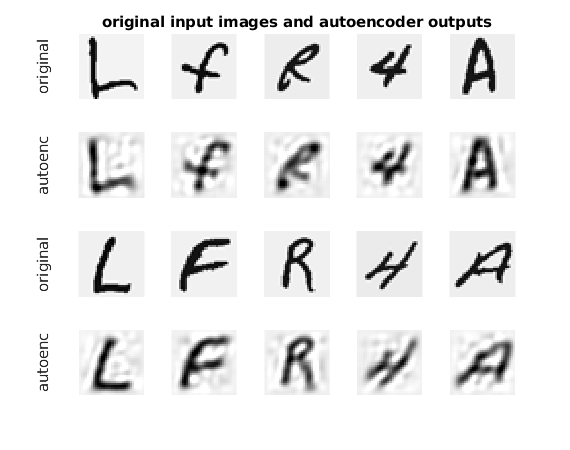
\includegraphics[page=1,width=0.75\textwidth]{q531_auto}
\caption{ Loss and RMSE for autoencoder training } 
\label{fig:autoencout}
\end{figure}   

\subsection{Q5.4}


\end{document}


